\documentclass[tikz]{standalone}
\begin{document}
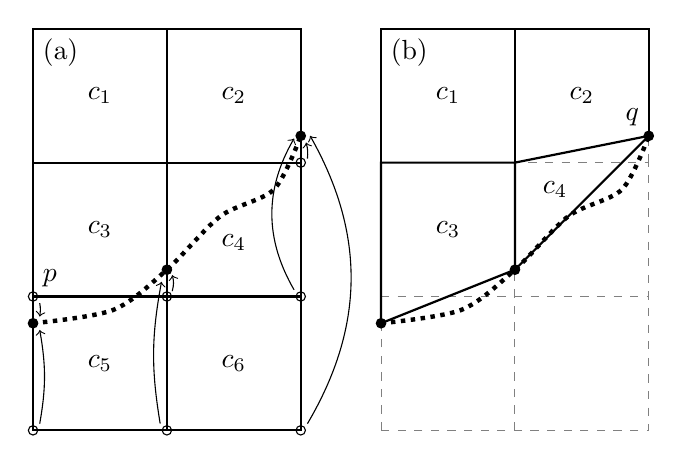
\begin{tikzpicture}[
  scale=0.17
]
\draw [thick] (0,0) rectangle (20, 20);
\draw [thick] (10,0) -- (10,20);
\draw [thick] (0,10) -- (20,10);
\draw [thick] (0,20) -- (0,30) -- (20,30) -- (20,20);
\draw [thick] (10,20) -- (10,30);
\draw [dotted, ultra thick] plot [smooth] coordinates {(0,8) (6, 9) (10,12) (14,16) (18,18) (20,22)};
\fill (0,8) circle [radius=0.4];
\fill (10,12) circle [radius=0.4];
\fill (20,22) circle [radius=0.4];
\draw (0,0) circle [radius=0.35];
\draw (0,10) circle [radius=0.35] node [anchor=south west] {$p$};
\draw (10,0) circle [radius=0.35];
\draw (10,10) circle [radius=0.35];
\draw (20,0) circle [radius=0.35];
\draw (20,10) circle [radius=0.35];
\draw (20,20) circle [radius=0.35];
\draw [->] (0.5,9.5) to [bend left=10] (0.5,8.5);
\draw [->] (0.5,0.5) to [bend right=10] (0.5,7.5);
\draw [->] (9.5,0.5) to [bend left=10] (9.6,11.1);
\draw [->] (10.4,10.4) to [bend right=15] (10.4,11.6);
\draw [->] (19.5,10.5) to [bend left=30] (19.5,21.8);
\draw [->] (20.5,0.5) to [bend right=30] (20.7,22);
\draw [->] (20.5,20.3) to [bend right=10] (20.4,21.5);
\node at (5,25) {$c_1$};
\node at (15,25) {$c_2$};
\node at (5,15) {$c_3$};
\node at (15,14) {$c_4$};
\node at (5,5) {$c_5$};
\node at (15,5) {$c_6$};

\node [below right] at (0,30) {(a)};

\draw [white] (20.6,0) rectangle (20.7,0);

\begin{scope}[shift={(26,0)}]
\draw [dashed, gray] (0,0) rectangle (20, 20);
\draw [dashed, gray] (10,0) -- (10,20);
\draw [dashed, gray] (0,10) -- (20,10);
\draw [dashed, gray] (20,20) -- (20,30);

\draw [thick] (0,8) -- (0,20) -- (10,20) -- (10,12) -- (0,8);
\draw [thick] (10,20) -- (20,22) -- (10,12);
\draw [thick] (0,20) -- (0,30) -- (20,30) -- (20,22);
\draw [thick] (10,20) -- (10,30);
\draw [dotted, ultra thick] plot [smooth] coordinates {(0,8) (6, 9) (10,12) (14,16) (18,18) (20,22)};
\fill (0,8) circle [radius=0.4];
\fill (10,12) circle [radius=0.4];
\fill (20,22) circle [radius=0.4] node [anchor=south east] {$q$};
\node at (5,25) {$c_1$};
\node at (15,25) {$c_2$};
\node at (5,15) {$c_3$};
\node at (13,18) {$c_4$};

\node [below right] at (0,30) {(b)};
\end{scope}
\end{tikzpicture}
\end{document}
